% Template for ICASSP-2017 paper; to be used with:
%          spconf.sty  - ICASSP/ICIP LaTeX style file, and
%          IEEEbib.bst - IEEE bibliography style file.
% --------------------------------------------------------------------------
\documentclass{article}
\usepackage{spconf,amsmath,amssymb,bm,graphicx}
\usepackage{multirow}
% Example definitions.
% --------------------
\def\x{{\mathbf x}}
\def\L{{\cal L}}

\makeatletter
 \newcommand{\rmnum}[1]{\romannumeral #1}
 \newcommand{\Rmnum}[1]{\expandafter\@slowromancap\romannumeral #1@}
\makeatother

% Title.
% ------
\title{Deep Convolutional-Deconvolutional Neural Network for Ultrasonic Tomography}
%
% Single address.
% ---------------
\name{Wenbo Zhao, Zhun Chen, Yuanwei Jin, Jos\'e M. F. Moura, Ming Li, Jimmy Zhu\thanks{Thanks to XYZ agency for funding.}}
\address{Author Affiliation(s)}
%
% For example:
% ------------
%\address{School\\
%	Department\\
%	Address}
%
% Two addresses (uncomment and modify for two-address case).
% ----------------------------------------------------------
%\twoauthors
%  {A. Author-one, B. Author-two\sthanks{Thanks to XYZ agency for funding.}}
%	{School A-B\\
%	Department A-B\\
%	Address A-B}
%  {C. Author-three, D. Author-four\sthanks{The fourth author performed the work
%	while at ...}}
%	{School C-D\\
%	Department C-D\\
%	Address C-D}
%
\begin{document}
%\ninept
%
\maketitle
%
\begin{abstract}

Ultrasonic tomography usually uses iterative methods to reconstruct images, which suffer heavy computation burden. Inspired by the beamforming technique, this paper presents an end-to-end neural network framework for ultrasonic tomography, which employs a convolutional-deconvolutional structure for fast image inferring from received signals. Simulations validate the effectiveness of the proposed framework with high inference accuracy and acceptable image quality.

\end{abstract}
%
\begin{keywords}

Ultrasonic tomography, Neural networks, Image reconstruction, Deep learning

\end{keywords}
%
\section{Introduction}
\label{sec:intro}

Ultrasonic tomography involves reconstructing the image by slices from ultrasound signals received by ultrasonic transducers after the signals probing through some medium. Conventional image reconstruction methods for ultrasonic tomography are iterative in nature, such as the algebraic reconstruction techniques (ART)\cite{gordon1974tutorial}, the simultaneous algebraic reconstruction technique (SART)\cite{andersen1984simultaneous}, the simultaneous iterative reconstruction technique (SIRT)\cite{trampert1990simultaneous}, the propagation and backpropagation method (PBP)\cite{dong2013mimo}. They are computationally expensive, and the iterations are repeated in each imaging process. We propose an end-to-end neural network approach for ultrasonic tomography, which allows for fast inference of images from received signals given the trained network. We adopt a deep convolutional-deconvolutional network structure with skip layers to fully capture the characteristics of the underlying wave propagation model, in which the stacked convolutional network performs multi-scale weighting to encode the input, and the stacked deconvolutional network decodes these higher layer representations into images. We train the proposed conv-deconv network on large dataset that takes the cross spectral matrix of the received signals as input, and the ground truth images as output. We validate the effectiveness of the conv-deconv network by computing the error of predicted images on test input.

% In beamforming where the plane wave assumption holds, it is possible to steer the probing to different locations in the imaging area to achieve high resolution at multiple locations. However, this approach need to perform expensive scan for each point on the image grid, an a proper setting for steering weights is crucial for good imaging quality, which in reality is hard to tune, and vulnerable to noise.

\subsection{Related Work}
\label{sub:related_work}

Literature shows that artificial neural networks (ANNs) have been used in solving the inverse problem of ultrasonic tomography for target detection\cite{anthony1992ultrasound,pardoe1997neural}. These approaches usually assume a simplified mathematical model for wave propagation, have low image resolution and quality, and use simple multilayer perception structure. More common applications are using neural networks for classifying and segmenting ultrasonic images\cite{dokur2002segmentation,sujana1996application,prater1992segmenting,feleppa2002ultrasonic}, in which deep learning structures, such as deep belief network\cite{carneiro2012segmentation}, are employed. These approaches do not generalize a wave propagation model, and are applications specific. Other applications involves using neural networks for ultrasound image enhancement and compression\cite{miller1992review}. We present an end-to-end, deep conv-deconv structured network that generalizes the wave propagation model, provide fast inference of high quality images over the input signals.

\subsection{Contributions}
\label{sub:contribution}
The contributions of this work are two-folded. Firstly, it provides an end-to-end neural network framework for fast inference of high quality images from ultrasonic signals with high accuracy. Secondly, it promotes a deep conv-deconv network structure that is able to fully generalize the characteristics of the underlying wave propagation model.

\section{Approach}
\label{sec:approach}

In this section, we derive the mathematical formulation of the generalized ultrasonic wave propagation and image reconstruction process, and present the conv-deconv network for solving the problem.

\subsection{Problem Formulation}
\label{sub:problem_formulation}

Consider using a linear array of $N$ ultrasonic transducers to transmit ultrasonic pulses to the medium under inspection and receive the responses. We assume the imaging region in the medium is formed by $\sqrt{L} \times \sqrt{L}$ rectangular grids, where $L$ is the total number of pixels in the image. The received signal $S_n(t)$ at time $t$ at the $n^{\mathbf{th}}$ transducer is represented by
\begin{equation}
	S_n(t) = \sum_i^M q_i(t)g_n(x_i) + b(t),
	\label{eq:received_signal}
\end{equation}
where $q_i$ is one of the $M$ sources, $g_n(x_i)$ is the Green's function specified at source location $x_i$ and for the receiving channel $n$, and $b$ is the additive noise. We consider the signals' frequency domain representations, and let $S_n(f)$ denote the Fourier transform of $S_n(t)$. In order to retrieve the source signal $q_i$ at the location $x_i$, we correlate $S_n$ by $g_n$ at an arbitrary location $x$ for each receivers, which yields\cite{dougherty2008beamforming}
\begin{equation}
	U_x(f) = \alpha\sum_n^N g_n(x)S_n(f),
	\label{eq:U_f} 
\end{equation}
where $\alpha$ is a multiplicative coefficient, and the value for $U_x(f)$ peaks when $x$ coincides with the source location $x_i$. This follows the power of $U_x$
\begin{equation}
	A_x = |U_x|^2 = \mathbf{g}(x)^*\left\langle \mathbf{S},\mathbf{S}^*\right\rangle \mathbf{g}(x),
	\label{eq:power}
\end{equation}
where $\langle\cdot\rangle$ is the average operator, and $\mathbf{g}(x)^*$ denotes the complex conjugate of $\mathbf{g}(x)$. We further collect the power $A_x$ for all possible $L$ locations in the image into a $\sqrt{L} \times \sqrt{L}$ matrix
\begin{equation}
	\mathbf{A} = \mathbf{W}^*\mathbf{C}\mathbf{W},
	\label{eq:vectorized_form}
\end{equation}
where $\mathbf{W}=\alpha\mathbf{g}$ is the unknown $N \times \sqrt{L}$ weight matrix, and $\mathbf{C}=\langle \mathbf{S},\mathbf{S}^* \rangle$ is the $N \times N$ cross spectral matrix. We generalize (\ref{eq:vectorized_form}) into
\begin{equation}
    \mathbf{A} = \mathcal{R}_{\mathbf{w}}(\mathbf{C}),
    \label{eq:generalized_form}
\end{equation}
where the nonlinear operator $\mathcal{R}_\mathbf{w}: H\rightarrow H_j$ maps from Hilbert space $H$ to $H_j$. Our objective is to find the optimal $\mathbf{W}$ that
\begin{equation}
	\widehat{\mathbf{W}} = \underset{\mathbf{W}}{\mathrm{argmin}}\,|\mathcal{R}_{\mathbf{w}}(\mathbf{C})-\mathbf{y}|^2,
	\label{eq:optimization_prob}
\end{equation}
where $\mathbf{y}$ is the ground truth of $\mathbf{A}$. We propose a neural network approach to solve (\ref{eq:optimization_prob}), as shown in next subsection.

\subsection{Deep Convolution-Deconvolution Network}
\label{sub:deep_conv-deconv_net}

We propose a convolutional-deconvolutional network structure that takes the cross spectral matrix (CSM) $\mathbf{C}$ of the received signals as input, and outputs image $\mathbf{A}$. The structure of the network is illustrated in Fig.~\ref{fig:net_structure}.
\begin{figure}[htbp]
  \centering
  \centerline{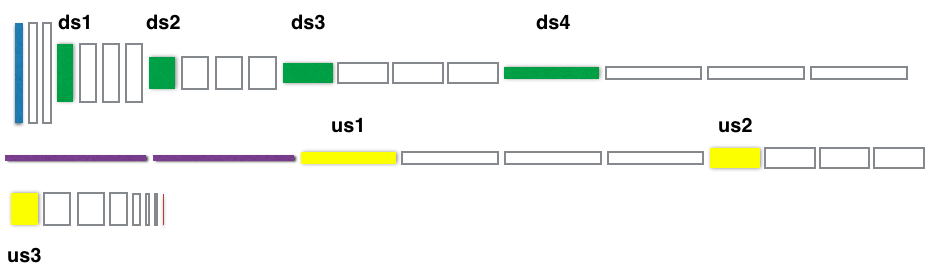
\includegraphics[width=8.5cm]{net_structure}}
\caption{Illustration of the conv-deconv network structure. The blue and red rectangles represent input and output. The green boxes represent down-sampling layers, and the yellow ones represent up-sampling layers. The rest are convolutional layers.}
\label{fig:net_structure}
\end{figure}
The former part of the network is constructed by a $N \times N \times R$ input layer followed by a sequence of convolutional layers, where $N$ and $R$ denote the number of channels in the receiver array and the number of angles in the scan. The configuration of these convolutional layers is shown in Tab.~\ref{tab:conv_config}.
\begin{table}[htbp]
\center
\caption{Configuration of convolutional layers}
  \begin{tabular}{ c | c c c c c c c c c c}
    \hline
    layer no. & 1 & 2 & 3 & 4 & 5 & 6 & 7 & 8 & 9 & 10 \\
    \hline
    filter size $F$ & \multicolumn{2}{c|}{5} & 4 & \multicolumn{3}{|c|}{3} & 4 & \multicolumn{3}{|c}{3} \\
    \hline
    no. of filters $D$ & \multicolumn{2}{c|}{64} & \multicolumn{4}{c|}{128} & \multicolumn{4}{c}{256} \\
    \hline
    padding size $P$ & \multicolumn{2}{c|}{2} & \multicolumn{8}{c}{1} \\
    \hline
    stride $S$ & \multicolumn{2}{c|}{1} & 2 & \multicolumn{3}{|c|}{1} & 2 & \multicolumn{3}{|c}{1} \\
    \hline
    activation $\delta$ & \multicolumn{10}{c}{ReLU} \\
    \hline
    \hline
    layer no. & 11 & 12 & 13 & 14 & 15 \\
    \hline
    filter size $F$ & 4 & \multicolumn{3}{|c|}{3} & 4 \\
    \hline
    no. of filters $D$ & \multicolumn{4}{c|}{512} & 1024 \\
    \hline
    padding size $P$ & \multicolumn{5}{c}{1} \\
    \hline
    stride $S$ & 2 & \multicolumn{3}{|c|}{1} & 2 \\
    \hline
    activation $\delta$ & \multicolumn{5}{c}{ReLU} \\
    \hline
  \end{tabular}
  \label{tab:conv_config}
\end{table}
We use the rectified linear unit (ReLU) as our activation function\cite{nair2010rectified}. We note that in replacement of using max-pooling layer as the down-sampling layer, which is adopted by many state-of-art convolutional architectures\cite{krizhevsky2012imagenet,simonyan2014very,long2015fully,szegedy2015going}, we use convolutional layers with stride $S=2$ to perform down-sampling. This allows the network to learn the down-sampling parameters by itself and leads to comparable results as using max-pooling layers\cite{springenberg2014striving}.

\subsubsection{Deconvolution}
\label{ssub:deconv}
The latter part of the conv-deconv network is constructud by a sequence of deconvolutional networks. Contrary to the convolutional layer that takes input of size $I \times I$ and yields output of size $O \times O$, where $O = (I-F+P)/2S + 1$, the deconvolution operation reverses what is done in the convolution via what is called \emph{transposed convolution}\cite{dumoulin2016guide} and outputs the shape of size $I \times I$ from input size $O \times O$\cite{zeiler2014visualizing}, and hence the deconvolutional network up-samples the output of the convolutional network. The configuration of the deconvolution layers is shown in Fig.~\ref{tab:deconv_config}.
\begin{table}[htbp]
\center
\caption{Configuration of deconvolutional layers}
  \begin{tabular}{ c | c c c c c c c c}
    \hline
    layer no. & 16 & 17 & 18 & 19 & 20 & 21 & 22 & 23 \\
    \hline
    filter size $F$ & \multicolumn{8}{c}{3} \\
    \hline
    no. of filters $D$ & 1024 & \multicolumn{4}{|c|}{512} & \multicolumn{3}{c}{256} \\
    \hline
    padding size $P$ & 1 & \multicolumn{1}{|c|}{3} & \multicolumn{3}{c|}{1} & 5 & \multicolumn{2}{|c}{1} \\
    \hline
    stride $S$ & \multicolumn{8}{c}{1} \\
    \hline
    activation $\delta$ & \multicolumn{8}{c}{ReLU} \\
    \hline
    \hline
    layer no. & 24 & 25 & 26 & 27 & 28 & 29 & 30 & 31 \\
    \hline
    filter size $F$ & \multicolumn{8}{c}{3} \\
    \hline
    no. of filters $D$ & 256 & \multicolumn{3}{|c|}{128} & 64 & 32 & 16 & 4 \\
    \hline
    padding size $P$ & 1 & \multicolumn{1}{|c|}{9} & \multicolumn{6}{c}{1} \\
    \hline
    stride $S$ & \multicolumn{8}{c}{1} \\
    \hline
    activation $\delta$ & \multicolumn{8}{c}{ReLU} \\
    \hline
  \end{tabular}
  \label{tab:deconv_config}
\end{table}
We note that this structure closely resembles the stacked autoencoders\cite{masci2011stacked,vincent2010stacked}, with a primary difference that autoencoders have their output the same with their input, and learn the compact representation of the input in the bottleneck layers (e.g. the layer 15 and 16 in Fig.~\ref{fig:net_structure}), while our proposed structure takes in the CSM and outputs an image. In another sense, we can treat the convolutional layers as stacked encoders that encode the input to its abstract representation, and the deconvolutional layer as stacked decoders that decode the abstract representation to image.

\subsubsection{Skip-Layer Structure}
\label{ssub:skip_layer}

We also employ the skip-layer structure to directly combine a deep, coarse layer with the information from a shallow, fine layer to produce accurate and detailed image reconstruction\cite{long2015fully}. Specifically, we directly sum the output of the down-sampling layer (layer \emph{ds4} in Fig.~\ref{fig:net_structure}) with the output of the up-sampling layer (layer \emph{us1}), and feed the summation layer to the convolutional layer after layer \emph{us1}. We then sum the output of layer \emph{ds3} and the output of layer \emph{us2}, and feed the summation layer to the layer after layer \emph{us2}.

\section{Simulations and Results}
\label{sec:simulations_results}

In the simulations, we use the specialized ultrasound simulation software package Field \Rmnum{2}\cite{}, and perform the network training and inference on Keras\cite{keras} framework with Theano\cite{theano2016short} backend.

\subsection{Simulation Setting}
\label{sub:simulation_setting}

In the simulation, we collect $T=7000$ images, and transform each of them to binary image by forcing pixel intensities greater than the mean intensity plus two times the standard deviation of the intensities to one, and the rest pixel intensities to zero. We use this collection of binary images $\mathbf{B}=\bigcup_{t=1}^{T}\{\mathbf{x}_t:x_i=1\,\mathrm{or}\,0, i=1,2,\ldots,L\}$ as ground truth images. A sample of the images is shown in Fig.~\ref{}. We use an array of 192 elements with the kerf\cite{} $0.0025\,\mathrm{mm}$. To generate the signal responses, we transmit a sine wave with the the center frequency $f_c=5\,\mathrm{MHz}$ and the sampling frequency $f_s=100\,\mathrm{MHz}$ to the medium $\mathbf{B}$. For each $\mathbf{x}_t\subset\mathbf{B}$, we impose a set of scatters with uniformly distributed positions and normally distributed amplitudes with zero mean and variance scaled by the variance of $\mathbf{x}_t$. We simulate the behavior of phased array by repeatedly steer the transmitted signal to the image plane from $-48$ degrees to $48$ degrees with $1.45$ degrees increment, total $66$ lines, in each transmission only $64$ elements being active. This generates the signal responses $\mathbf{S}$ of dimension $64 \times K \times 66$ for each $\mathbf{x}_t$, with $K$ being the length of the signal responses. An illustration of the received signals for 64 channels at steering angle $??$ is shown in Fig.~\ref{}.

\subsection{Training Network and Inference}
\label{sub:training_inference}

The input for training the network is the CSM $\mathbf{C}$ computed from the generated signal responses $\mathbf{S}$ over a total $7000$ samples, which is a 4D tensor of dimension $7000 \times 66 \times 64 \times 64$. The output for training the network is the corresponding image collection $\mathbf{B}$. In the training, we randomly shuffle the training set with 10 percent of the training set as validation set. The specific training configuration is shown in Tab.~\ref{tab:train_config}.
\begin{table}[htbp]
\center
\caption{Training configuration}
  \begin{tabular}{ c | c }
    \hline
    batch size $B_s$ & 100 \\
    \hline
    no. epoch $E_p$ & 5000 \\
    \hline
    learning rate $\gamma$ & 0.01 \\
    \hline
    learning rate decay $\eta$ & 0.0005 \\
    \hline
    momentum $m$ & 0.9 \\
    \hline
    loss $L_e$ & MSE \\
    \hline
  \end{tabular}
  \label{tab:train_config}
\end{table}
We use the mean square error (MSE) to measure the error between the predicted images and the ground truth images.
The plot of training error $\epsilon$, cross validation error $r$ with regard to the number of iterations is illustrated in Fig.~\ref{}. It shows that \ldots 
% \begin{figure}[htbp]
Using the trained network, we now predict the images over a test set containing $1000$ CSMs computed from $1000$ additional signal responses generated from the images not in $\mathbf{B}$. Fig.~\ref{} shows the plot of error with regard to the number of iterations. It shows that \ldots Tab.~\ref{} shows the metrics of accuracy.

\section{Conclusions}
\label{sec:conclusions}


% \section{ILLUSTRATIONS, GRAPHS, AND PHOTOGRAPHS}
% \label{sec:illust}

% Illustrations must appear within the designated margins.  They may span the two
% columns.  If possible, position illustrations at the top of columns, rather
% than in the middle or at the bottom.  Caption and number every illustration.
% All halftone illustrations must be clear black and white prints.  Colors may be
% used, but they should be selected so as to be readable when printed on a
% black-only printer.

% Since there are many ways, often incompatible, of including images (e.g., with
% experimental results) in a LaTeX document, below is an example of how to do
% this \cite{Lamp86}.

% Below is an example of how to insert images. Delete the ``\vspace'' line,
% uncomment the preceding line ``\centerline...'' and replace ``imageX.ps''
% with a suitable PostScript file name.
% -------------------------------------------------------------------------
% \begin{figure}[htbp]

% \begin{minipage}[b]{1.0\linewidth}
%   \centering
%   \centerline{\includegraphics[width=8.5cm]{image1}}
% %  \vspace{2.0cm}
%   \centerline{(a) Result 1}\medskip
% \end{minipage}
% %
% \begin{minipage}[b]{.48\linewidth}
%   \centering
%   \centerline{\includegraphics[width=4.0cm]{image3}}
% %  \vspace{1.5cm}
%   \centerline{(b) Results 3}\medskip
% \end{minipage}
% \hfill
% \begin{minipage}[b]{0.48\linewidth}
%   \centering
%   \centerline{\includegraphics[width=4.0cm]{image4}}
% %  \vspace{1.5cm}
%   \centerline{(c) Result 4}\medskip
% \end{minipage}
% %
% \caption{Example of placing a figure with experimental results.}
% \label{fig:res}
% %
% \end{figure}


% To start a new column (but not a new page) and help balance the last-page
% column length use \vfill\pagebreak.
% -------------------------------------------------------------------------
%\vfill
%\pagebreak

% \section{COPYRIGHT FORMS}
% \label{sec:copyright}

% You must submit your fully completed, signed IEEE electronic copyright release
% form when you submit your paper. We {\bf must} have this form before your paper
% can be published in the proceedings.

% \section{RELATION TO PRIOR WORK}
% \label{sec:prior}

% The text of the paper should contain discussions on how the paper's
% contributions are related to prior work in the field. It is important
% to put new work in  context, to give credit to foundational work, and
% to provide details associated with the previous work that have appeared
% in the literature. This discussion may be a separate, numbered section
% or it may appear elsewhere in the body of the manuscript, but it must
% be present.

% You should differentiate what is new and how your work expands on
% or takes a different path from the prior studies. An example might
% read something to the effect: "The work presented here has focused
% on the formulation of the ABC algorithm, which takes advantage of
% non-uniform time-frequency domain analysis of data. The work by
% Smith and Cohen \cite{Lamp86} considers only fixed time-domain analysis and
% the work by Jones et al \cite{C2} takes a different approach based on
% fixed frequency partitioning. While the present study is related
% to recent approaches in time-frequency analysis [3-5], it capitalizes
% on a new feature space, which was not considered in these earlier
% studies."

\vfill\pagebreak

% \section{REFERENCES}
% \label{sec:refs}

% List and number all bibliographical references at the end of the
% paper. The references can be numbered in alphabetic order or in
% order of appearance in the document. When referring to them in
% the text, type the corresponding reference number in square
% brackets as shown at the end of this sentence \cite{C2}. An
% additional final page (the fifth page, in most cases) is
% allowed, but must contain only references to the prior
% literature.

% References should be produced using the bibtex program from suitable
% BiBTeX files (here: strings, refs, manuals). The IEEEbib.bst bibliography
% style file from IEEE produces unsorted bibliography list.
% -------------------------------------------------------------------------
\bibliographystyle{IEEEbib}
\bibliography{refs}

\end{document}
